\documentclass{article}

\usepackage{sourcecodepro}
\usepackage{fontenc}
\usepackage{xcolor}
\usepackage{listings}
\usepackage{cite}
\usepackage[margin=1in]{geometry}
\usepackage{scrextend}
\usepackage{hyperref}
\hypersetup{
	colorlinks=true,
	linkcolor=blue,
	linktoc=page
}
\definecolor{mGreen}{rgb}{0,0.6,0}
\definecolor{mGray}{rgb}{0.5,0.5,0.5}
\definecolor{mPurple}{rgb}{0.58,0,0.82}
\definecolor{backgroundColour}{rgb}{0.95,0.95,0.92}
\definecolor{remColor}{rgb}{0.8,0.4,0.4}
\lstdefinestyle{Cpp}{
	backgroundcolor=\color{backgroundColour},
	commentstyle=\color{mGreen},
	keywordstyle=\color{magenta},
	numberstyle=\tiny\color{mGray},
	stringstyle=\color{mPurple},
	basicstyle=\footnotesize\ttfamily,
	breakatwhitespace=false,
	breaklines=true,
	captionpos=b,
	keepspaces=true,
	numbers=left,
	numbersep=5pt,
	showspaces=false,
	showstringspaces=false,
	showtabs=false,
	tabsize=4,
	language=C++
}

\def \bs {\textbackslash}

\def \cpp #1 {
	\lstinputlisting[style=Cpp]{cpp/#1}
}
\def \cpprng #1#2#3 {
	\lstinputlisting[style=Cpp, firstline=#2, lastline=#3]{cpp/#1}
}

\def \rem #1 {\iftrue{
	\textcolor{remColor}{
		\begin{addmargin}{2em}
			\small{Remark: #1}
		\end{addmargin}
	}
} \fi}



\title{COMP2123 self-learning report \\
Unit testing}
\author{Chan Kwan Yin (3035466978), Lee Chun Yin (3035469140)}

\begin{document}

\rem{TODO: Change \bs{}iftrue in commands.tex \bs{}def\bs{}rem to \bs{}iffalse in final copy}
\rem{In case we don't have enough content, just add more code examples, and maybe compare specific unit testing frameworks in some frameworks.}
\rem{Talking about CI (continuous integration) platforms like Travis-CI is also possible}
\newpage

\pagenumbering{roman}

\maketitle
\begin{abstract}
This report discusses the motivation, available techniques and difficulties of unit testing.
\end{abstract}
\newpage

{\hypersetup{hidelinks}
	\tableofcontents
}
\newpage

\pagenumbering{arabic}

\section{What is unit testing?}
Instead of just running the program and seeing if the output is correct,
unit testing splits down a software into small components and checks if the desired behaviour of each component is correct.


\section{Motivation}
\subsection{Discover bugs early}
As the scale of a software project grows, debugging becomes more complicated.
It may take a long time to discover edge case bugs in an old component, which is very difficult to debug after a long time.
Unit testing allows identification of bugs as soon as possible with little impact.

\subsection{As a method of specification}
Unit testing can also be used as a means of project requirement specification.


\section{Unit testing methods}
\subsection{Testing for expected result}
The intuitive way is to write a test that tests the output of each function.

If we have a \texttt{fooBar.cpp} with the following definition:

\cpp{fooBar.cpp}

To ensure \texttt{fooBar()} always return \texttt{"qux"}, we can write a test to test this behaviour:

\cpp{fooBar.test.cpp}

The \texttt{ASSERT\_EQUAL} macro function would compare the result of \texttt{fooBar()} with \texttt{"qux"} and trigger an error if they are not equal.
This macro function can be implemented very easily:

\cpp{assert.h}

In this implementation, if the values are not equal, an exception string is thrown.

Different unit testing frameworks may have different error behaviour, and some are able to integrate with IDEs for advanced analysis.

Some other common assertions include:
\begin{itemize}
	\item Null checks
	\item Arithmetic comparisons $<$ $\leq$ $>$ $\geq$
	\item That an expected exception must be thrown
\end{itemize}

By running a series of similar tests every time before moving to another project subcomponent,
bugs can be identified before it spreads to other components.
This is particularly helpful when certain bugfixes might result in prototype changes,
resulting in incompatibility with other components during bugfixes.

\subsection{Increasing the test size}
If a function accepts parameters, multiple calls with different values should be passed to the function.

Suppose we want to test a function that converts a number to scientific notation rounded to 3 significant figures:

\cpp{sciNot1.cpp}

Testing the simple case of rounding $1235$ to $124\times10^1$ is successful:

\cpp{sciNot1.test.cpp}
\cod{sciNot1.log}

However, adding more test parameters, such as negative inputs, would turn out that the function does not always function as expected:

\cpp{sciNot2.test.cpp}
\cod{sciNot2.log}

From this, we can identify that a negative input results in a negative value, apparently because of the \texttt{log10} function call.
So a simple workaround of fixing the input to a positive number can be made:

\cpp{sciNot3.cpp}
\cod{sciNot3.log}

\subsection{Generating test cases randomly}
Since a larger test size is more likely to catch bugs, it is a good idea to generate a large sample of test cases.

Generating random test cases also avoids the case where a developer is writing specific test cases (e.g. only multiples of 7)
to avoid unit tests from reflecting a known bug in the code.

\subsubsection{Random output, inverse-evaluated input}
But a contradictory condition arises: If the test cases are generated, how to test if the result is correct?
It is not possible to calculate the value in the test generator, because that would involve reimplementing the tested function.

Instead, if an inverse of the tested function can be written
(or to generate any of the possible inverse values if the function is not an injection),
the random generator can be used to generate random results instead.

Nevertheless, the inverse function is often harder to write and likely to have bugs than the function to test for,
and is usually unintuitive to be used as a way of software specification.
A better approach is to use property-based testing.

\subsubsection{Property-based testing}
Instead of comparing if the output is equal to an expected result,
property-based testing compares the characteristics of the output to determine if it is reasonable.

In C++, the \href{https://github.com/emil-e/rapidcheck}{rapidcheck} library
provides a property-based testing framework that generates a random sequence of data by type for assertion.

For example, in the 3-sigifnicant-figure example above, the requirements are:

\begin{enumerate}
	\item Given an input $n$, the output $\hat{n} = d \times 10^{x}$ is returned.
	\item The result significand $d$ must have exactly 3 significant figures, i.e. $d \in [100, 999]$
	\item The error must be correct to the \nth{3} significant figure: $\hat{n} - n \in [-0.5 \times 10^{x}, 0.5 \times 10^{x})$
\end{enumerate}

The \nth{1} requirement is defined through the function prototype,
and the \nth{2} and \nth{3} requirements can be specified by the following test:

\cpp{sciNot5.test.cpp}
\cod{sciNot5.log}

\subsubsection{Reimplement algorithm by brute-force}
Even though the test only expresses the software specification, it may still be difficult to implement.
Suppose the following function is specified:

\begin{itemize}
	\item Parameter \texttt{int n}: the number of nodes
	\item Parameter \texttt{vector<pair<int, int>> edges}: each pair is two numbers indicating two node IDs of a directed edge.
	\item Node IDs are integers in the range $[0, n)$.
	\item If a Hamiltonian circuit is present, return any possible \texttt{vector<int> *} such that
		the node IDs in the vector represent a Hamiltonian circuit for the graph.
	\item If a Hamiltonian circuit is not present, return \texttt{NULL}.
\end{itemize}

Assume the function is implemented in a certain polynomial-time algorithm
(which is possible given more specifications on the graph,
but it is omitted as Hamiltonian circuit algorithm is not the focus of this project).

While it is simple to test for the correctness for returned vectors, it is very difficult to test if returning \texttt{NULL} is correct.
The specification "Hamiltonian circuit is not present" is very well-defined, but it is still not possible to validate.
In this case, a brute-force approach can be used to test for the correctness.

Although the function was implemented in an efficient polynomial-time algorithm, tests do not strictly require a high performance.
It is therefore appropriate to test the new algorithm
with a potentially less error-prone and more reliable algorithm using brute-force, i.e. NP time.
This is because unit tests do not have to be tolerant of large data;
light-weightedness is one of the core concepts of unit testing.
(Stress testing is another topic not related to unit testing)

\subsubsection{Testing for edge cases}
\rem{E.g. test for empty strings, Float.INFINITY, 0, etc.}


\section{Unit testing techniques}
\subsection{Test coverage}
Test coverage is a criterion to assess the representativeness of the unit tests of a project by counting the number of lines executed in the test.

\rem{Talk about the integration of debuggers and how to interpret coverage (codecov.io)}

\subsection{Test-driven development (TDD)}
As a consequence of unit testing, development flow becomes more fluent if each development subtask is based on certain test cases. By using TDD, it ensures that every part of the program can be tested properly, as nearly all code is writen based on pre-written test cases. It also prevents writing duplicated code in large collaborative projects, and TDD can avoid waste of time for implmenting already done features/requirements. 

The workflow of TDD is as follows:

\begin{enumerate}
	\item Create a new unit test for the software for a requirement that has not yet been implemented. 
	\item Run the unit test. If the unit test passes, this means the new test overlaps with previously written tests, and that a new test should be written to cover the new requirement
	\item Write code to pass (only) the newly added test, while ensuring previous tests also pass
	\item Run the tests
	\item Repeat the above process for every requirement
\end{enumerate}

Suppose we want to write a calulator with a fucntion \texttt{int add(string numbers)} that has the following requirements:

\begin{enumerate}
	\item The method can take in any amount of space-separated integers as an input, and return their sum.
	\item If the string is empty, the method should return \texttt{0}.
	\item If non-space-and-digit characters are passed within the string, the method throw an "Invalid character" exception. 
\end{enumerate}

We begin the development process by writing the test for the first requirement as follows:

\rem C++ test

As the \texttt{sum} method is currently empty, the test fails as expected. So we can proceed to write the code which solves this test:

\cpp{calculator1.cpp}

To verify our implementation, we run the test we have written in test 1:

\rem{Run test, success}

And we can continue with implementing the next requirement. 

\textbf{Exercise: Write the test and implementation for the second test.}

\subsection{Behaviour-driven development (BDD)}

While TDD provides a reliable method to test individual function executions, it cannot precisely and concisely define functions that depend on global/object states.

The main difference between TDD and BDD is that while TDD ensures that every sub-component of the software is correct, BDD provides a more "high-level" view of what the entire software should provide to the user. It is often regarded as a "bridge" between product designers and developers, as through BDD, product designers can effectively communicate their needs to devlopers who specialize in implementing those requirements. 

BDD defines the behaviour of a function using some specific terms or keywords. Each of these is written in the format of a "user story", and follow special "syntax" via the usage of certain keywords. The usage of these keywords are important, as a user story can be automatically phrased into "testable" code with a framework (such as Cucumber, on next section), given that it is formatted correctly with those "grammar". Here we present some of the keywords, along with the syntax general to most BDD frameworks:

The following is an example BDD of Cucumber:

\begin{lstlisting}
Feature: Is it Friday yet?
  Everybody wants to know when it's Friday

  Scenario: Sunday isn't Friday
    Given today is Sunday
    When I ask whether it's Friday yet
    Then I should be told "Nope"
\end{lstlisting}

\paragraph{Feature}

Describes a feature that the software should provide on the high-level, with some description

\paragraph{Scenario}

Describes a situation (similar to example) where that the software should be able to handle properly, defines the behavior of the program for a certain (more specific) situation. 

\paragraph{Given}

The initial state of the program when this scenario takes place

\paragraph{When}

Similar to natural English, "When" implies that the following statement should be done "when" this statement is completed

\paragraph{Then}

Describes the expected output of the program after the preceeding "when" statement is fulfilled. 

Why is such grammar important? As a software developer, we may often find it difficult to translate requirements given by product designers/users into code. By having the product designers write their requirements in such a fashion which is both "human readable" and "machine prasable", it is possible to translate those requirements in to unit tests \textbf{automatically}. For example, in Cucumber, the following can be generated automatically from the above BDD, which can be further manipulated to contain actual machine-runnable tests (in fact a BDD is just a combination of multiple unit tests, but written in a high-level manner):

\java{cucumber_unit_test.java}

If you are interested to learn more, head over to \url{http://docs.cucumber.io/guides/10-minute-tutorial/} to get started with the Cucumber framework!

\subsection{Summary: TDD vs BDD}

As you can see, the description of the program behavior in BDD is more "high level" compared to TDD. The person writing BDDs ususally writes them from a user's perspective, where they might not have full knowledge on the internals of the software. On the other hand, TDDs focus more on the internal working on the software, and whether each part functions correctly. 

Often in BDD, when a test fails, it is difficult to locate the root cause of the error, as the BDD usually involves the whole piece of software instead of a single modular component and it is difficult to locate a bug in the whole program as opposed to a single function. (in Cucumber, the framework subclassifies a task into multiple components to help to identify the exact source of error, but the subclassification is not as small as those in TDD). Furthermore, as BDD involves running the whole software to conduct behavior tests, it takes much longer to conduct a single test (a BDD test can take up to a minute, while a TDD test may only take a few seconds). 

The existence of BDDs is to keep developers on track on building products that directly address the user's requirements, instead of building functions that satisfy a low-level requirement. This means, that in BDD the software development is driven by how the user will use the software, and the program is built accordingly, while for TDD, it involves the concept where the correctness of a software implies that all sub-components are correctly writen, meaning that code is built according to the feature of a certain component, but not the whole picture. 

This means if a BDD test fails, it implies that there is a use case that the software will have a bug in regular use, and should not be released. On the other hand, if BDD passes and a TDD fails, this implies that although some components may contain bugs, in regular usage, they will not affect the running of the whole software, and the software can continue with its release, leaving the bug fix for later. 

\subsection{Dependency mocking}

Often (if not always), sub-components in a software will have other components as dependencies. Take our calculator class as an example. Suppose we want to write a function \texttt{int eval(int a, int b, char operation)}

\cpp{calculator2.cpp}

The implementation is done, and we have unit tests for this code. Now lets say that there is a new requirement, that if the result of the calculation exceeds the value of \texttt{int} (2^{31}-1), it should throw an OverflowException. A trivial idea for implementation would be to implement the internal calcualtion of the operation via another data type that supports larger range (e.g. \texttt{long long}, \texttt{BigInteger}), and compare this value with 2^{31}-1. In other words, we can write the following instead:

\cpp{calculator3.cpp}

The \texttt{Calculator} now depends on \texttt{BigInteger}. Assume that we have not implemented or tested our implementation of \texttt{BigInteger} yet, how are we going to test the component of \texttt{Calculator}? One of the ways is to substitute \texttt{BigInteger} with another "fake" BigInteger, which for the purpose of explanation, we assume the implementation is correct.

\cpp{Fake_BigInteger.h}

Now our \texttt{Calculator} class can compile successfully, and we can test the implementation of \texttt{Calculator} without caring about the correctness of \texttt{BigInteger}. 

This is exactly what "Dependency mocking" is. If inside the target we want to perform unit tests on, has a function call which either is untested, or we do not want to call (due to lack of resources, take long time to run), we can essentially substitute that function with another one which produces the "expected result" of the original function, assuming that the implementation of the original function was correct. Mocking is useful when it is impractical to call a function many time during the testing stage of development, such as those which consume a lot of time like database calls. 

However, although mocking effectively isolates the target component from other components, making unit testing relevant to the implementation of only the target, mocking has several disadvantages for software development. By essentially "negelecting" the implementation of other components, it makes the target component prone to unexpected behavior of the target component. For instance, if there were any updates to the dependencies, such as a new exception being thrown, the current unit tests would not be aware of such new behavior, and the tests may not be accurate. For example, the unit test may run successfully with mocks, but with the actual "unmocked" implementation, it has a runtime error, and the developer may be unaware to this. This is particularly important in large projects with many dependencies, perhaps with dependencies not being written by the in-house developers, and it is difficult to update mocks to fully reflect the current behavior of the dependencies. 

If you want to know more about mocking and its advantages/disadvantages, check out \url{https://enterprisecraftsmanship.com/2016/06/09/styles-of-unit-testing/}. 

\section{Difficulties}

\subsection{Coupling}
Coupling is the cyclic dependency between units to be tested.

In large software projects, components are usually dependent on one another.
For example, the dependency graph of a web server might look like figure \ref{fig:depweb}.

\begin{figure}
	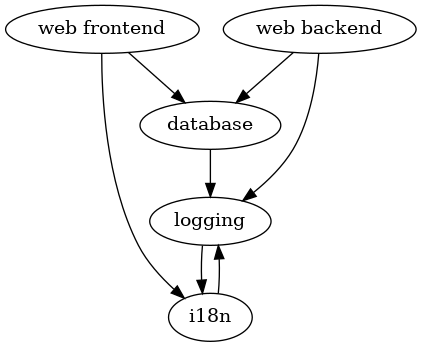
\includegraphics[width=3in]{example-deps.png}
	\caption{Dependency graph of a web server}
	\label{fig:depweb}
\end{figure}

A relation worth noting is between logging and i18n.
I18n requires a logger to log its loading process,
and logger requires i18n to display proper messages.
While this is complicated to write from the beginning,
it is even harder to unit test,
because it is not possible to only unit test logger without having a functional i18n component.

In other words, it is not possible to decide which component to unit test first,
because both modules are mutually dependent.

This condition is called modular coupling. Common practices to prevent it include:

\paragraph{Abstraction}: Create an interface for logger and simulate a simple dummy logger to unit test i18n.
Create an interface for i18n and simulate a constant dummy i18n system to unit test logger.
\paragraph{Dependency mocking}As explained in the previous section, dependency mocking can be used to prevent dependencies while testing,
but there are many problems about dependency mocking too.

Therefore, the best solution to coupling is to prevent cyclic dependencies from the beginning.


\section{Sources}
The source for building this report and all test cases can be found at \url{https://github.com/chankyin/comp2123-project}

\end{document}
